% beam_template.tex
\documentclass[a4paper,10pt]{article}
\usepackage[left=20mm,right=20mm,top=25mm,bottom=25mm,bindingoffset=0mm]{geometry}
\usepackage{fontspec}
\usepackage{fancyhdr}
\usepackage{graphicx}
\usepackage[detect-all=true]{siunitx}
\usepackage{stanli}
\usepackage{amsmath}
\usepackage{booktabs}
\usepackage{tikz}
\usepackage{calc}
\usepackage{xcolor}
\usepackage{adjustbox}


\pagestyle{fancy}
\fancyhead[L]{\small Katedra Wytrzymałości Materiałów, WILiŚ, PG}
\fancyhead[R]{\small rok. akad. 2025/2026}
\fancyfoot[L]{\textcolor{gray}{\textit{Numer zadania (do informacji sprawdzającego): 782000}}}
\fancyfoot[C]{}

\begin{document}

    \begin{center}
    {\Large \textbf{Podstawy Mechaniki Komputerowej - Projekt}}
    \end{center}

    \begin{table}[ht]
        \centering
        \begin{tabular}{
            m{.175\textwidth}m{.215\textwidth}m{.175\textwidth}m{.175\textwidth}m{.1\textwidth}}
        \toprule
        Imię & Nazwisko & Numer albumu & Numer grupy  & Ocena \\ \midrule
             &          &              &              &       \\ \bottomrule
        \end{tabular}
        \label{tab:dane_studenta}
    \end{table}

    \noindent\textbf{Treść zadania:} \vspace{1mm}

    Dla przedstawionego układu prętowego należy:

    \begin{itemize}
        \item Wyznaczyć wykresy sił wewnętrznych: sił tnących \(T\) oraz momentów zginających \(M\), \textbf{przedsta\-wione w odpowiednich jednostkach}.
        \item Sporządzić \textbf{rysunek} deformacji układu, oznaczając \textbf{wartości charakterystyczne ugięć} oraz uwzględniając \textbf{obliczone kąty obrotu}.
    \end{itemize}

    Zadanie należy rozwiązać, stosując \textbf{Macierzową Metodę Przemieszczeń} i element belkowy. W analizie numerycznej proszę wykorzystać bibliotekę \textbf{CalFEM} w środowisku \textbf{MATLAB}. Poniższa tabela zawiera dane niezbędne do realizacji zadania:

    \begin{table}[ht]
    \centering
    \renewcommand{\arraystretch}{1.25}
    \begin{tabular}{lllllll}
    \toprule
    Długość [\si{m}] &
                $L_{1} = 3$ &                $L_{2} = 5$ &                $L_{3} = 3$ &                $L_{4} = 4$ &                $L_{5} = 4$ &                $L_{6} = 5$             \\
    Moduł Younga [\si{GPa}] &
                $E_1 = 190$ &                $E_2 = 200$ &                $E_3 = 190$ &                $E_4 = 200$ &                $E_5 = 190$ &                $E_6 = 30$             \\
    Moment bezwładności [\si{\centi\meter^4}] &
                $I_1 = 3217$ &                $I_2 = 1018$ &                $I_3 = 27440$ &                $I_4 = 2492$ &                $I_5 = 8000$ &                $I_6 = 833$             \\
    \bottomrule
    \end{tabular}
    \label{tab:dane_zadania2}
    \end{table}

    Na zadany układ działają następujące obciążenia w postaci
 sił skupionych
        $P_1 = 30 \si{\kilo\newton}$%
,         $P_2 = 5 \si{\kilo\newton}$%
    ,
 momentów zginających
        $M_1 = 20 \si{\kilo\newton m}$
,         $M_2 = 4 \si{\kilo\newton m}$
    oraz
 obciążeń liniowych
        $q_1 = 7 \si{\kilo\newton/\meter}$%
,         $q_2 = 1 \si{\kilo\newton/\meter}$%
    .

    \vspace{5mm}

    \noindent\textbf{Schemat układu:}

    \begin{center}
    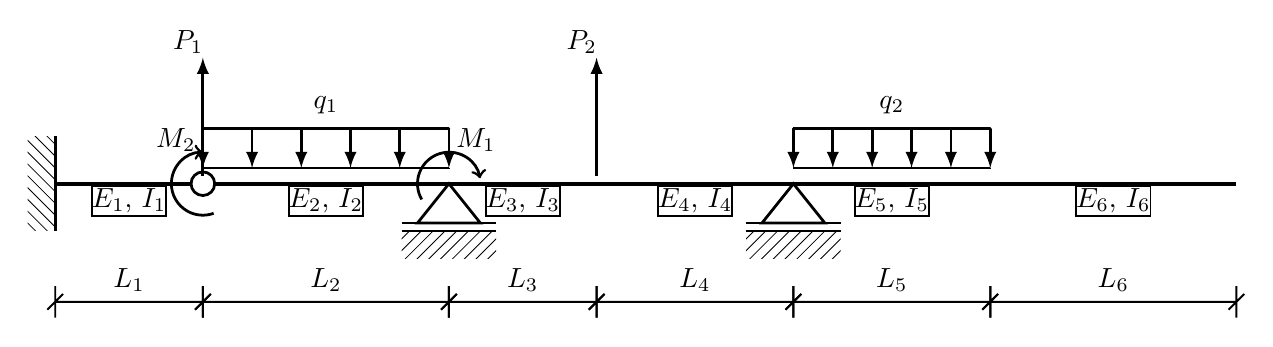
\begin{tikzpicture}[x=0.625cm, y=1cm]
    % nodes definition
        \point{n1}{0.0}{0.0}
        \point{n2}{3.0}{0.0}
        \point{n3}{8.0}{0.0}
        \point{n4}{11.0}{0.0}
        \point{n5}{15.0}{0.0}
        \point{n6}{19.0}{0.0}
        \point{n7}{24.0}{0.0}
    % elements definition
        \beam{2}{n1}{n2}
        \notation{4}{n1}{n2}[$E_1$, $I_1$][0.5][below=.2mm];
        \dimensioning{1}{n1}{n2}{-1.5}[$L_1$]
        \beam{2}{n2}{n3}
        \notation{4}{n2}{n3}[$E_2$, $I_2$][0.5][below=.2mm];
        \dimensioning{1}{n2}{n3}{-1.5}[$L_2$]
        \beam{2}{n3}{n4}
        \notation{4}{n3}{n4}[$E_3$, $I_3$][0.5][below=.2mm];
        \dimensioning{1}{n3}{n4}{-1.5}[$L_3$]
        \beam{2}{n4}{n5}
        \notation{4}{n4}{n5}[$E_4$, $I_4$][0.5][below=.2mm];
        \dimensioning{1}{n4}{n5}{-1.5}[$L_4$]
        \beam{2}{n5}{n6}
        \notation{4}{n5}{n6}[$E_5$, $I_5$][0.5][below=.2mm];
        \dimensioning{1}{n5}{n6}{-1.5}[$L_5$]
        \beam{2}{n6}{n7}
        \notation{4}{n6}{n7}[$E_6$, $I_6$][0.5][below=.2mm];
        \dimensioning{1}{n6}{n7}{-1.5}[$L_6$]
    % supports definition
        \support{3}{n1}[-90]
        \support{2}{n3}[0]
        \support{2}{n5}[0]
    % hinges definition
        \hinge{1}{n2}
    % loads definition
        \lineload{3}{n2}{n3}[0.5][0.5][-0.1]
        \coordinate (midpoint) at ($ (n2)!0.5!(n3) $);
        \node[fill=white, fill opacity=0.8, text opacity=1, inner sep=1pt] at (midpoint) [shift={(0, 1)}] {$q_1$};
        \lineload{3}{n5}{n6}[0.5][0.5][-0.1]
        \coordinate (midpoint) at ($ (n5)!0.5!(n6) $);
        \node[fill=white, fill opacity=0.8, text opacity=1, inner sep=1pt] at (midpoint) [shift={(0, 1)}] {$q_2$};
        \load{1}{n2}[-90][1.5][-1.6]
        \node[fill=white, fill opacity=0.8, text opacity=1, inner sep=1pt] at (n2) [shift={(-0.3, 1.5 + 0.3)}] {$P_1$};
        \load{1}{n4}[-90][1.5][-1.6]
        \node[fill=white, fill opacity=0.8, text opacity=1, inner sep=1pt] at (n4) [shift={(-0.3, 1.5 + 0.3)}] {$P_2$};
        \node[fill=white, fill opacity=0.8, text opacity=1, inner sep=1pt] at (n3) [shift={(0.55, 0.55)}] {$M_1$};
        \load{2}{n3}[10][200]
        \node[fill=white, fill opacity=0.8, text opacity=1, inner sep=1pt] at (n2) [shift={(-0.55, 0.55)}] {$M_2$};
        \load{2}{n2}[90][200]
    \end{tikzpicture}
    \end{center}

    \vspace{5mm}

    \noindent\textbf{Wymagane elementy opracowania:}

    \begin{enumerate}
    \item Rysunek dyskretyzacji układu \dotfill 5 pkt
    \item Skrypt w MATLAB-ie rozwiązujący zadanie (*.m) \dotfill 5 pkt
    \item Wykresy sił wewnętrznych: siły tnące \(T\) [\si{\kilo\newton}] i momenty zginające \(M\) [\si{\kilo\newton m}] \dotfill 10 pkt
    \item Rysunek deformacji układu [\si{\centi\meter}] \dotfill 5 pkt
    \end{enumerate}

    \vspace{5mm}

    \noindent\textbf{Uwagi:}
    \begin{itemize}
    \item Rysunek dyskretyzacji, wykresy sił tnących, momentów zginających oraz rysunek deformacji należy umieścić na odwrocie karty projektowej.
    \item Skrypt rozwiązujący zadanie należy przesłać do odpowiedniego modułu na platformie eNauczanie w ramach kursu \textit{Podstawy Mechaniki Komputerowej}.
    \item Nieprzesłanie skryptu skutkuje przyznaniem 0 punktów za elementy opracowania nr 3 i 4.
    \end{itemize}

\end{document}